\let\negmedspace\undefined
\let\negthickspace\undefined
\documentclass[journal]{IEEEtran}
\usepackage[a5paper, margin=10mm, onecolumn]{geometry}
%\usepackage{lmodern} % Ensure lmodern is loaded for pdflatex
\usepackage{tfrupee} % Include tfrupee package

\setlength{\headheight}{1cm} % Set the height of the header box
\setlength{\headsep}{0mm}     % Set the distance between the header box and the top of the text

\usepackage{gvv-book}
\usepackage{gvv}
\usepackage{cite}
\usepackage{amsmath,amssymb,amsfonts,amsthm}
\usepackage{algorithmic}
\usepackage{graphicx}
\usepackage{textcomp}
\usepackage{xcolor}
\usepackage{txfonts}
\usepackage{listings}
\usepackage{enumitem}
\usepackage{mathtools}
\usepackage{gensymb}
\usepackage{comment}
\usepackage[breaklinks=true]{hyperref}
\usepackage{tkz-euclide} 
\usepackage{listings}
% \usepackage{gvv}                                        
\def\inputGnumericTable{}                                 
\usepackage[latin1]{inputenc}                                
\usepackage{color}                                            
\usepackage{array}                                            
\usepackage{longtable}                                       
\usepackage{calc}                                             
\usepackage{multirow}                                         
\usepackage{hhline}                                           
\usepackage{ifthen}                                           
\usepackage{lscape}
\begin{document}

\bibliographystyle{IEEEtran}

\title{7.4.30}
\author{EE25BTECH11023 - Venkata Sai}
% \maketitle
% \newpage
% \bigskip
\maketitle \vspace{-1.5cm}
\renewcommand{\thefigure}{\theenumi}
\renewcommand{\thetable}{\theenumi}
\setlength{\intextsep}{10pt} % Space between text and floats

\numberwithin{align}{enumi}
\numberwithin{figure}{enumi}
\renewcommand{\thetable}{\theenumi}

\textbf{Question:}  \\
A circle is given by $x^2+(y - 1)^2=1$, another circle C touches it externally and also the $X$ axis, then the locus of its centre is
\begin{multicols}{2}
\begin{enumerate}[leftmargin =*]
    \item $\{\brak{x,y} : x^2 = 4y\} \cup \{(x,y) : y \leq 0\}$
    \item $\{\brak{x,y} : x^2+(y-1)^2 = 4\} \cup \{(x,y) : y \leq 0\}$
    \item $\{\brak{x,y} : x^2 = 4y\} \cup \{(0,y) : y \leq 0\}$
    \item $\{\brak{x,y} : x^2 = 4y\} \cup \{(0,y) : y \leq 0\}$
\end{enumerate}
\end{multicols}
\textbf{Solution:}  \\
As the circle touches $X-$axis , Distance of a point from $x$-axis is given by
\begin{align}
    r=|\vec{n}^\top\vec{c}|
\end{align}
where $\vec{n}$ is the unit vector normal to $x$-axis\\
For the given circle with radius $r_1$ and center $c_1$
\begin{align}
 x^2+(y - 1)^2=1\\
 \vec{p}=\myvec{0\\1}=\vec{n}\ \text{and}\ r_1=1 
\end{align}
Distance between their centers equal to sum of their radius
\begin{align}
    \norm{\vec{c}-\vec{p}}&=r+r_1\\
\norm{\vec{c}-\vec{n}}&=|\vec{n}^\top\vec{c}|+1 \\
\norm{\vec{c}-\vec{n}}^2&=\brak{|\vec{n}^\top\vec{c}|+1}^2 
\end{align}
\begin{align}
\brak{\vec{c}-\vec{n}}\brak{\vec{c}^\top-\vec{n}^\top}=\brak{|\vec{n}^\top\vec{c}|+1}^2 
\end{align}
\begin{align}
\vec{c}^\top\vec{c}+\vec{n}\vec{n}^\top-\vec{c}^\top\vec{n}-\vec{n}^\top\vec{c}&= \brak{|\vec{n}^\top\vec{c}|}^2+2|\vec{n}^\top\vec{c}|+1\\
\vec{c}^\top\vec{c}+\vec{n}\vec{n}^\top-\vec{c}^\top\vec{n}-\vec{n}^\top\vec{c}&=\brak{\vec{n}^\top\vec{c}}^\top\brak{\vec{n}^\top\vec{c}}+2|\vec{n}^\top\vec{c}|+1\\
\vec{c}^\top\vec{c}+\norm{\vec{n}}^2-2\vec{n}^\top\vec{c}&=\brak{\vec{c}^\top\vec{n}\vec{n}^\top\vec{c}}+2|\vec{n}^\top\vec{c}|+1 
\end{align}
\begin{align}
\vec{c}^\top\vec{c}+1&=\brak{\vec{c}^\top\vec{n}\vec{n}^\top\vec{c}}+2\vec{n}^\top\vec{c}+2|\vec{n}^\top\vec{c}|+1 
\end{align}
\begin{align}
\vec{c}^\top\vec{c}-\brak{\vec{c}^\top\vec{n}\vec{n}^\top\vec{c}}=2\vec{n}^\top\vec{c}+2|\vec{n}^\top\vec{c}| \\
\vec{c}^\top\brak{\vec{I}-\vec{n}\vec{n}^\top}\vec{c}=2\vec{n}^\top\vec{c}+2|\vec{n}^\top\vec{c}| 
\end{align}
\begin{align}
\vec{c}^\top\brak{\myvec{1&0\\0&1}-\myvec{0\\1}\myvec{0&1}}\vec{c}=2\myvec{0\\1}^\top\vec{c}+2\left|\myvec{0\\1}^\top\vec{c}\right| \\
\vec{c}^\top\brak{\myvec{1&0\\0&1}-\myvec{0&0\\0&1}}\vec{c}=2\myvec{0&1}\vec{c}+2\left|\myvec{0&1}\vec{c}\right|\\
\myvec{x&y}\brak{\myvec{1&0\\0&0}}\myvec{x\\y}=2\myvec{0&1}\myvec{x\\y}\pm2\myvec{0&1}\myvec{x\\y}
\end{align}
\begin{align}
\myvec{x&0}\myvec{x\\y}=4\myvec{0&1}\myvec{x\\y}\ \brak{\textbf{or}}\ \myvec{x&0}\myvec{x\\y}=2\myvec{0&1}\myvec{x\\y}-2\myvec{0&1}\myvec{x\\y}
\end{align}
\begin{align}
\myvec{x&0}\myvec{x\\y}=4y\ \brak{\textbf{or}}\ \myvec{x&0}\myvec{x\\y}=0 
\end{align}
\begin{align}
x^2=4y\ \brak{\text{or}}\ x^2=0 \implies x=0
\end{align}
Case \brak{1}
\begin{align}
x^2=4y \implies y\geq0
\end{align}
Case \brak{2}
\begin{align}
x&=0\\ 
\vec{n}^\top\vec{c}\leq0 \implies& \myvec{0&1}\myvec{x\\y} \leq 0 \implies y\leq 0
\end{align}
Hence from Case \brak{1} and Case \brak{2}
\begin{align}
    \cbrak{\brak{x,y}:x^2=4y} \bigcup \cbrak{\brak{x,y}:x=0\ \text{AND}\ y\leq0}
\end{align}
\begin{align}
    \cbrak{\brak{x,y}:x^2=4y} \bigcup \cbrak{\brak{0,y}:y\leq0}
\end{align}
\begin{figure}[H]
   \centering
   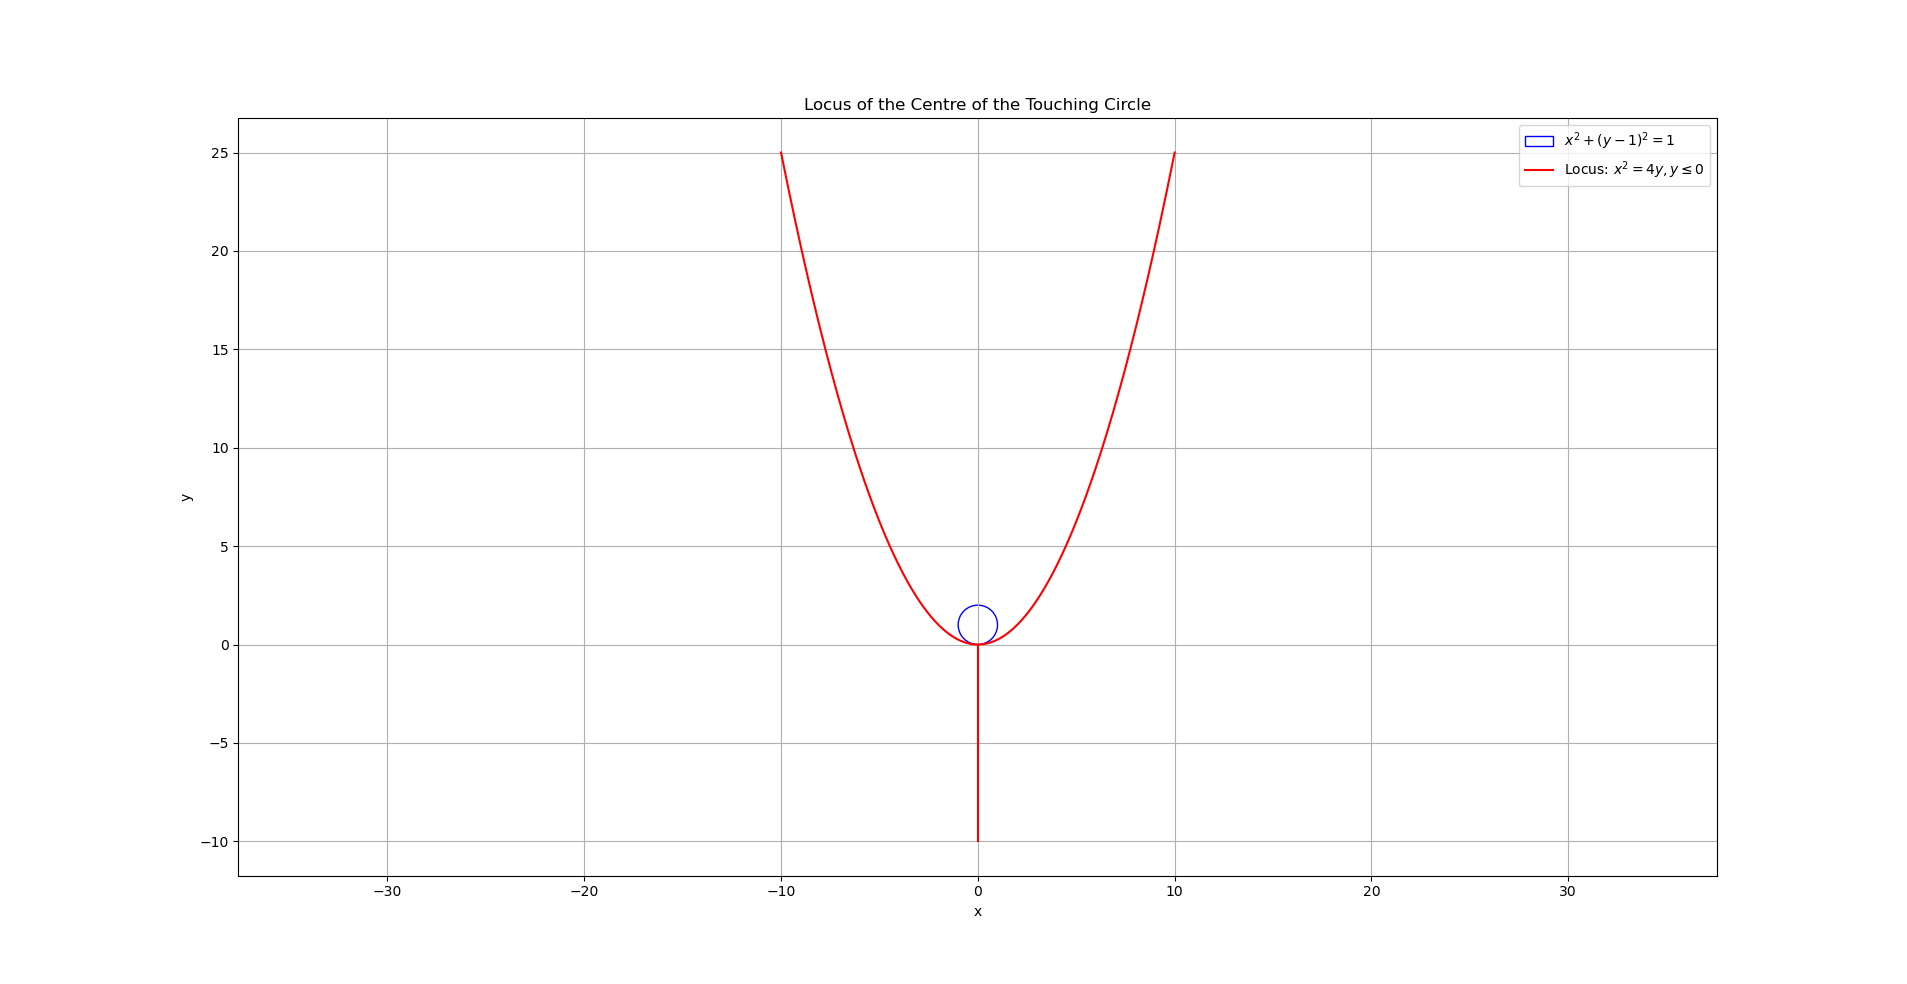
\includegraphics[width=0.7\columnwidth]{figs/fig1.png}
	\caption{}
   \label{}
\end{figure}
\end{document}  